\begin{figure}[t]
\centering
\subfigure{\centering 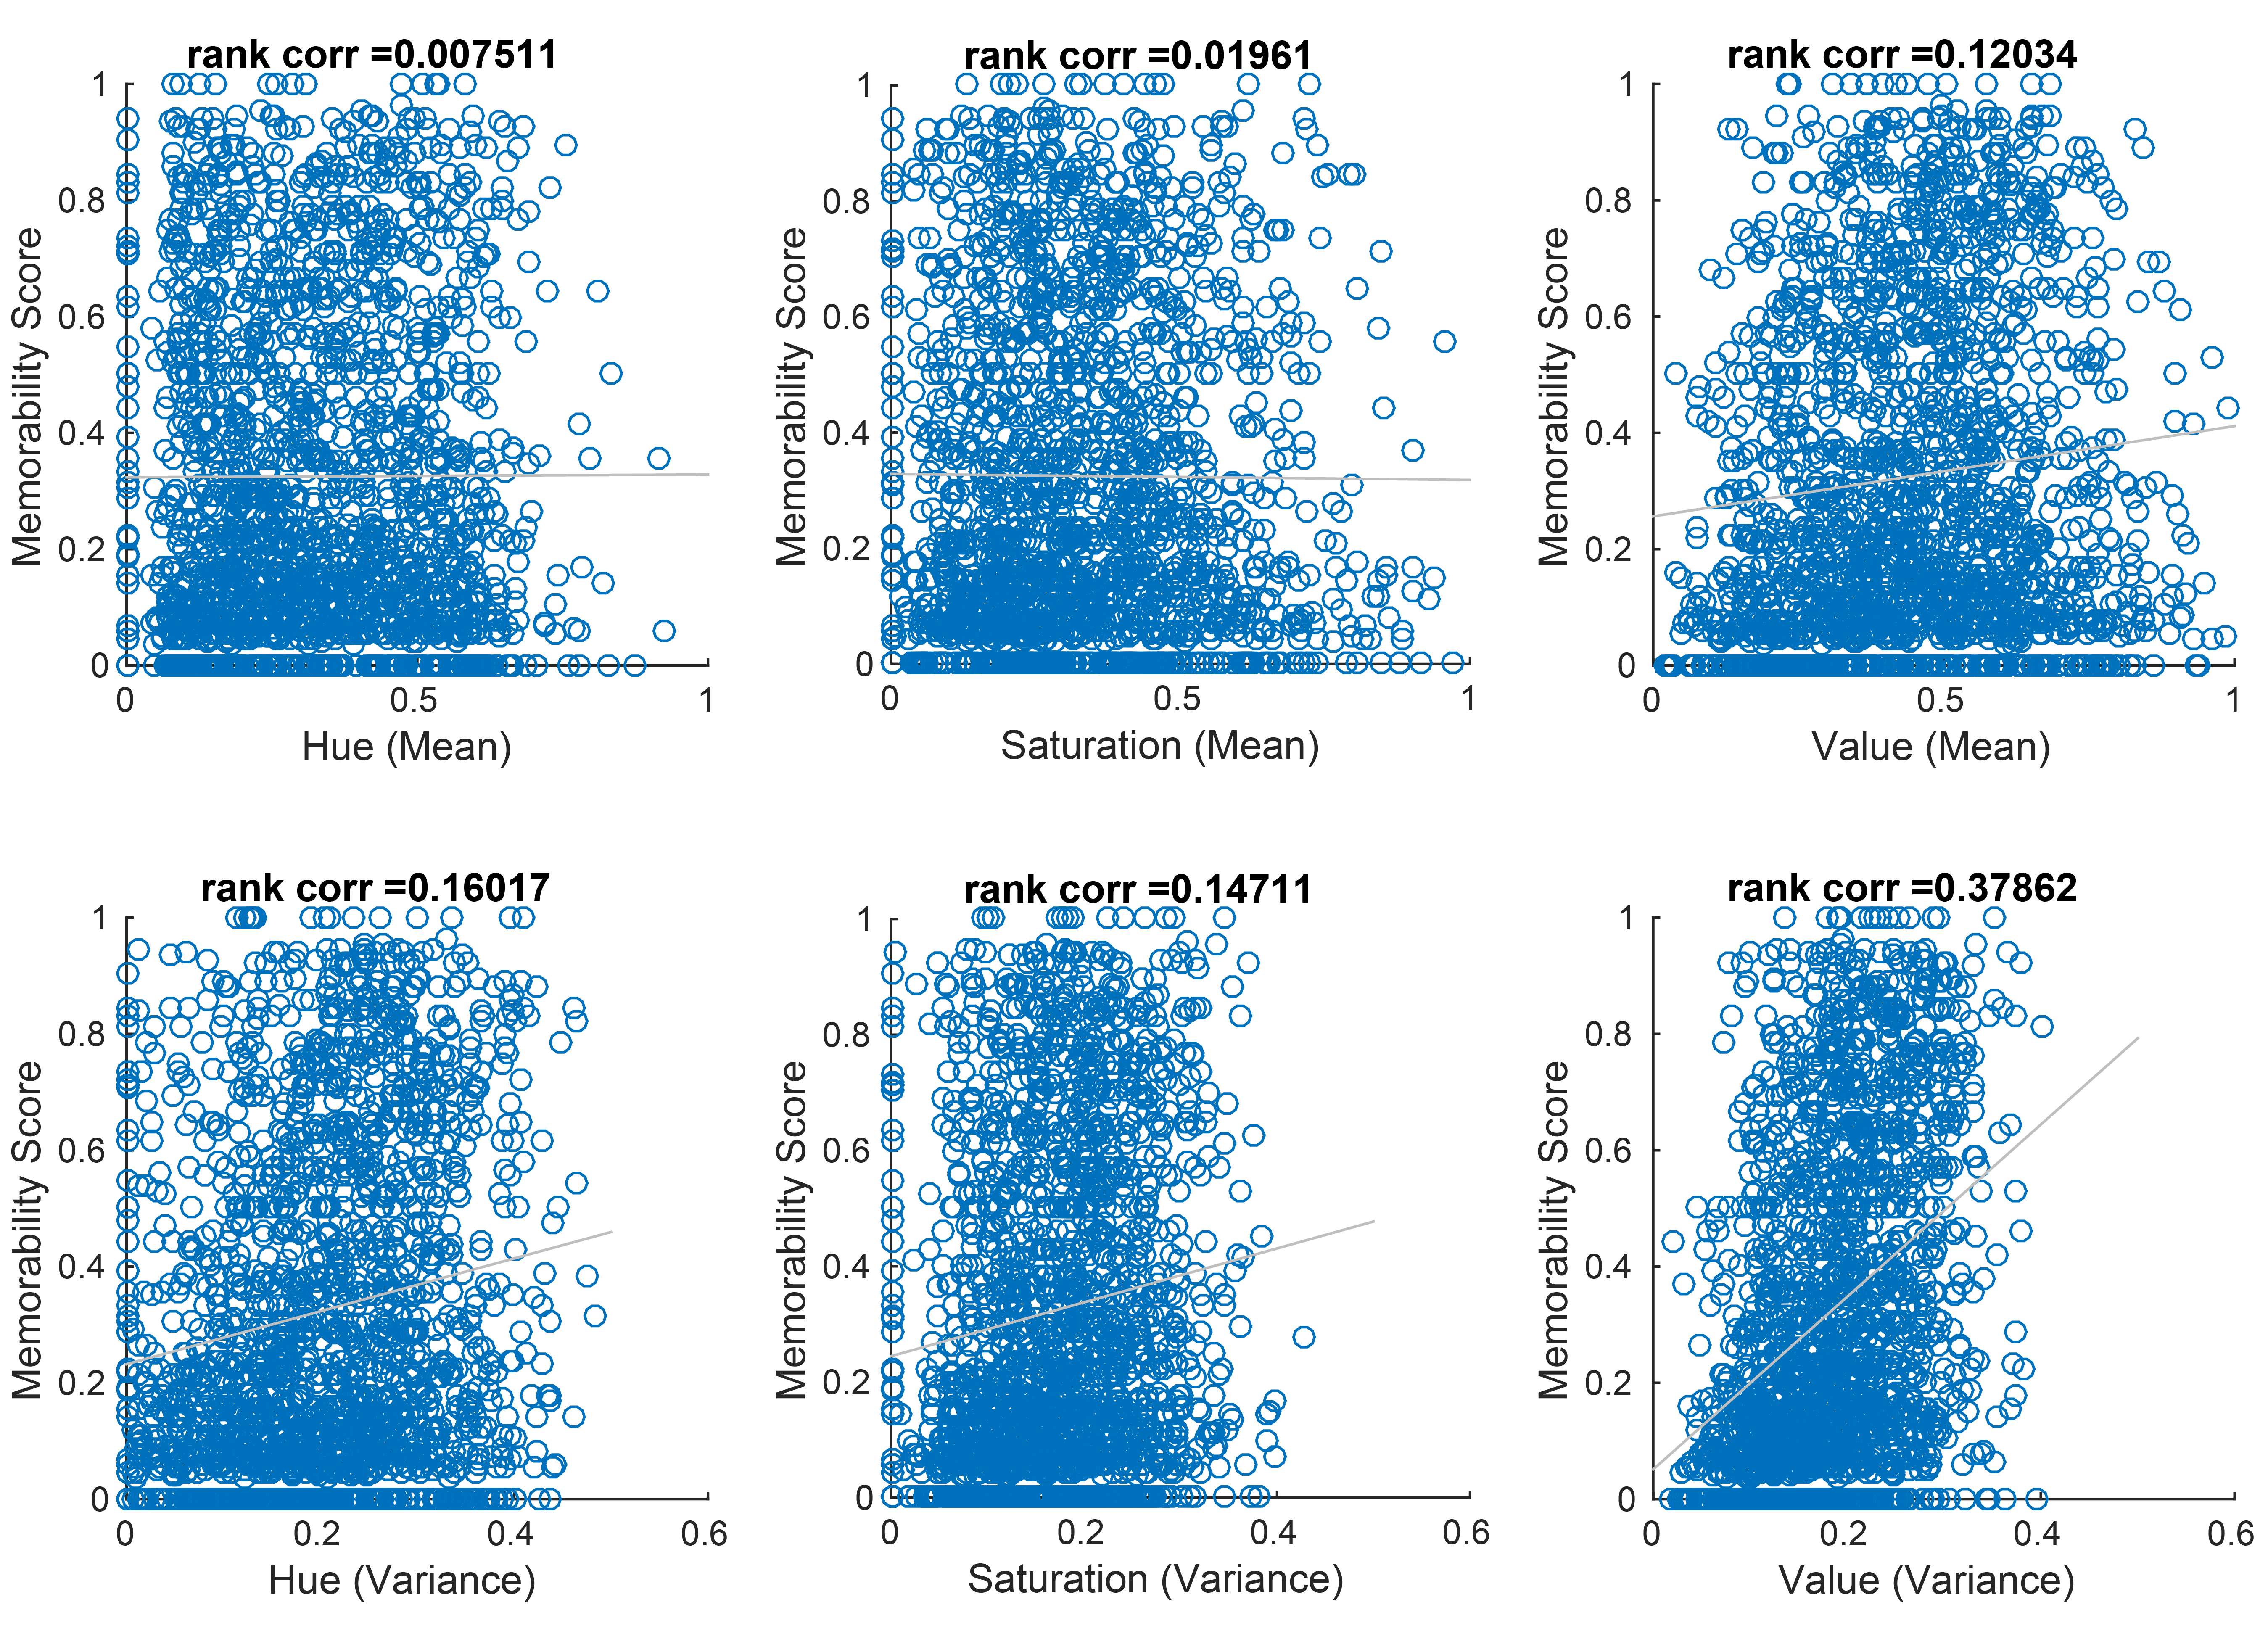
\includegraphics[width=\textwidth]{figures/results/corrs.png}}
\vspace{-5mm}\caption{\footnotesize\textbf{Correlations between simple color features and object memorability.} Color features were computed from HSV representations of the objects. }\label{fig:simple}
\end{figure}

While simple image features are traditionally poor predictors of memorability in full images [Oliva, CVPR 2011], and with good reason [cite [11] from Oliva, CVPR 2011]], it is important to verify that this finding generalizes to individual objects. To do this, we first examined a number of simple color statistics. We decomposed each image into it's hue, saturation, and value components and calculated the mean and standard deviation of each channel. Essentially no relationship existed between memorability and either mean hue (ρ = 0) or mean saturation (ρ = 0.02). This deviates somewhat from the findings related to images that show hue to be weakly predictive of memorability. However, this makes sense since the effect has been speculated to be due to the blue and green outdoor landscapes being less memorable than warmly colored human faces and indoor scenes. While our dataset contained plenty of indoor objects and people, outdoor scene-related image regions such as sky and ground were not included as objects. This may explain why the effect was not present in our dataset. Looking at the variance of each channel, we see that variance in hue (ρ = 0.16) and saturation (ρ = 0.15) are weakly correlated with memorability, while value has a medium correlation (ρ = 0.38). This suggests that variation in the color hue and color purity of an object contribute somewhat to object memorability. This may be because people are memorable regardless of the color of their clothing, or simply that color inhomogeneity draws ones attention. The finding that variation in value contributes considerably to object memorability indicates that high contrast objects are more memorable. Although the correlation seems high compared the the performance of past simple features in past research, the scatterplot in FIGURE X suggests that it may not produce reliable predictions. Next, we computed image size, calculated by the number of pixels that make up the object normalized by the total number of pixels in the parent image. Not surprisingly, this metric correlated strongly with object memorability (ρ = 0.53). This makes sense given that large objects, especially that take up the majority of the parent image frame, are more likely to be seen and identified. 